\begin{frame}{Главные ориентиры}
	\begin{itemize}
		\item кроссплатформенная переносимость
		\item открытые стандарты
	\end{itemize}
\end{frame}

\begin{frame}{Немного цитат}
Дуг Макилрой, изобретатель каналов <<pipes>>, сформулировал несколько постулатов,применимых для разработки ПО:
\pause
	\begin{itemize}
		\item пишите программы,  которые выполняют одну функцию и делают это хорошо;
			\pause
		\item пишите программы,  которые будут работать вместе;
			\pause
		\item пишите программы,  поддерживающие текстовые потоки,  поскольку они являются универсальным интерфейсом.
	\end{itemize}

\end{frame}


\begin{frame}{"Философия" UNIX}
	это {\bfseries не} философия,  а общие рекомендации по проектированию ПО,  накопленные сообществом программистов на опыте десятилетий разработок программ,  которые взаимодействуют друг с другом.
\end{frame}

\begin{frame}{1. Правило модульности}
	\begin{block}{Следует писать простые части,  связанные ясными интерфейсами.}
Единственным способом создания сложной программы,  не обреченной заранее на провал,  является сдерживание ее глобальной сложности.
	\end{block}
Т.е. построение программы из простых частей, соединенных четко определенными интерфейсами, 
так что большинство проблем являются локальными, 
и тогда можно рассчитывать на обновление одной из частей без разрушения целого.
\end{frame}

\begin{frame}{Размер кода и ошибки}
	\begin{center}
		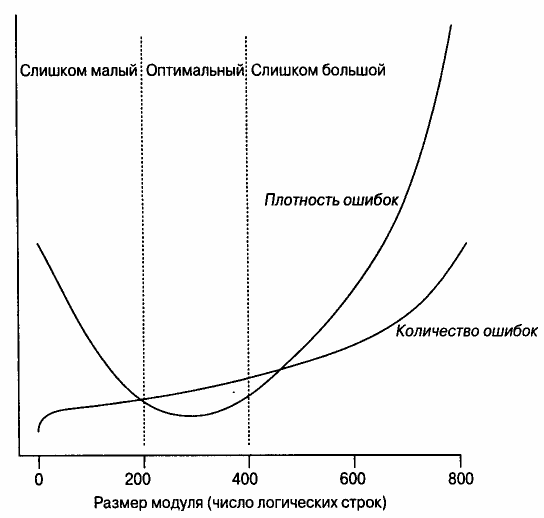
\includegraphics[width=200px]{../../slides/intro/errors_density-graph.png}
	\end{center}
\end{frame}

\begin{frame}{2. Правило ясности}
	\begin{block}{Ясность -- лучше чем мастерство.}
		Последующее обслуживание программы -- важная и дорогостоящая часть жизненного цикла программы.
	\end{block}
	\pause
Писать программы необходимо так,  как если бы вы знали,  что последующей поддержкой будет заниматься неуравновешенный псих с топором,  знающий ваш домашний адрес!
\end{frame}

\begin{frame}{3. Правило композиции}
	\begin{block}{Следует разрабатывать программы,  которые будут взаимодействовать с другими программами.}
		Если разрабатываемые программы не способны взаимодействовать друг с другом,  то очень трудно избежать создания сложных монолитных  программ.
	\end{block}
	Методы взаимодействия могут быть сильными и слабыми -- по возможности рекомендуется использовать слабые методы и текстовые форматы передачи данных.
\end{frame}

\begin{frame}{4. Правило разделения}
	\begin{block}{Следует отделять политику от механизма и интерфейсы от основных модулей (engine).}
		Примеры политики и механизма:\\
		вид GUI и операции отрисовки, клиент (front-end) -- сервер (back-end), сценарии и библиотеки и др.
	\end{block}
	При жесткой связи политики и механизма:
	\begin{itemize}
		\item политика становится негибкой и усложняется ее изменение;
		\item изменение политики имеет строгую тенденцию к дестабилизации механизмов.
	\end{itemize}
\end{frame}

\begin{frame}{5. Правило простоты}
	\begin{block}{Необходимо проектировать простые программы и <<добавлять сложность>> только там,  где это необходимо.}
	\end{block}
	Основные причины добавления сложности:
	\begin{itemize}
		\item человеческий фактор (часто -- желание <<выпендриться>>);
		\item проектные требования,  продиктованные текущей модой,  маркетингом или «левой пяткой заказчика»;
	\end{itemize}
\end{frame}

\begin{frame}{6. Правило расчетливости}
	\begin{block}{Пишите большие программы,  только если после демонстрации становится ясно,  что ничего другого не остается.}
		Под <<большими программами>> здесь понимаются программы с большим объемом кода и значительной внутренней сложностью.
	\end{block}
\end{frame}

\begin{frame}{7. Правило прозрачности}
	\begin{block}{Для того,  чтобы упростить проверку и отладку программы,  ее конструкция должна быть обозримой.}
		Программа {\itshape прозрачна}, если при ее минимальном изучении можно понять, что она делает и как.\\
		Программа {\itshape воспринимаема},  когда она имеет средства для мониторинга и отображения внутреннего состояния.
	\end{block}
	Необходимо использовать достаточно простые форматы входных и выходных данных.\\
	Интерфейс должен быть приспособлен для использования в отладочных сценариях.
\end{frame}

\begin{frame}{8. Правило устойчивости}
	\begin{block}{Устойчивость -- следствие	прозрачности и простоты.}
		Программа является {\itshape устойчивой},  когда она выполняет свои функции в неожиданных условиях,  которые выходят за рамки предположений разработчика,  как и в нормальных условиях.\\
		Программа является {\itshape простой},  если происходящее в ней не представляется сложным для восприятия человеком.
	\end{block}
	Один из способов организации -- модульность(простые блоки,  ясные интерфейсы)\\
	Следует избегать частных случаев!
\end{frame}

\begin{frame}{Пример неусточивого ПО}
	\begin{center}
		
\includegraphics[width=1\textwidth]{../../slides/intro/exploits_of_a_mom_rus.png}
	\end{center}
\end{frame}


\begin{frame}[fragile]{Пример <<простой>> программы}
	\begin{center}
		\begin{verbatim}
+++++++++++++++++++++++++++++++++++++++++++++
+++++++++++++++++++++++++++.+++++++++++++++++
++++++++++++.+++++++..+++.-------------------
---------------------------------------------
---------------.+++++++++++++++++++++++++++++
++++++++++++++++++++++++++.++++++++++++++++++
++++++.+++.------.--------.------------------
---------------------------------------------
----.-----------------------.
		\end{verbatim}
	\end{center}
\end{frame}

\begin{frame}{9. Правило представления}
	\begin{block}{Знания следует оставлять в данных,  чтобы логика программы могла быть примитивной и устойчивой.}
		Даже простую логику бывает сложно проверить,  но даже сложные структуры данных являются довольно простыми для моделирования и анализа (например диаграмма 50 узлов дерева и блок-схема 50 строк кода)
	\end{block}
	Если можно выбирать между усложнением структуры данных и усложнением кода,  то лучше выбирать первое.\\
	Примеры: ascii,  генератор html-таблицы.
\end{frame}

\begin{frame}{10. Правило наименьшего удивления}
	\begin{block}{При проектировании интерфейсов всегда следует использовать наименее неожиданные элементы.}
		Необходимо учитывать характер предполагаемой аудитории и традиции платформы.
	\end{block}
	Оборотная сторона: следует избегать создания внешне похожих вещей,  слегка отличающихся в действительности,  поскольку {\itshape кажущаяся привычность порождает ложные ожидания}.
\end{frame}

\begin{frame}{11. Правило тишины}
	\begin{block}{Если программе нечего сказать,  то пусть лучше молчит.}
		Внимание и сосредоточенность пользователя -- ценный и ограниченный ресурс,  который требуется только в случае необходимости.
	\end{block}
	Важная информация не должна смешиваться с подробными сведениями о работе программы.
\end{frame}

\begin{frame}{12. Правило восстановления}
	\begin{block}{Когда программа завершается аварийно,  это должно происходить явно (шумно) и по возможности быстро.}
		Если программа не способна справиться с ошибкой,  то необходимо завершить ее работу так,  чтобы максимально упростить диагностику.
	\end{block}
	Для сетевых служб следует следовать рекомендации Постела:\\
	<<{\itshape Будьте либеральны к тому,  что принимаете,  и консервативны к тому,  что отправляете}>>
\end{frame}

\begin{frame}{13. Правило экономии}
	\begin{block}{Время программиста дорого -- поэтому задача экономии его времени более приоритетна,  по сравнению с экономией машинного времени.}
		Компьютер железный -- ему не скучно (с) программистская мудрость
	\end{block}
	Использование высокоуровневых языков и <<обучение>> машины выполнять больше низкоуровневой работы по программированию,  что приводит к правилу 14.
\end{frame}

\begin{frame}{14. Правило генерации}
	\begin{block}{Избегайте кодирования вручную; если есть возможность -- пишите программы для создания программ.}
		Использование генераторов кода оправданно,  когда они могут повысить уровень абстракции,  
		т.е. когда язык спецификации для генератора проще,  чем сгенерированный код,  
		и код впоследствии не потребует ручной доработки.
	\end{block}
	Примеры: грамматические и лексические анализаторы,  генераторы make-файлов,  построители GUI-интерфейсов.
\end{frame}

\begin{frame}{15. Правило оптимизации}
	\begin{block}{Сначала -- опытный образец,  потом -- оптимизирование.}
		Добейтесь стабильной работы,  только потом оптимизируйте.
	\end{block}
	\begin{block}{Керниган и Плоджер:}
		90\% актуальной и реальной функциональности лучше,  чем 100\% функциональности перспективной и сомнительной
	\end{block}
	\begin{block}{Кнут:}
		преждевременная оптимизация -- корень всех зол
	\end{block}
	\begin{block}{Кент Бек (экстремальное программирование):}
		заставьте программу работать,  заставьте работать ее верно,  а затем сделайте ее быстрой
	\end{block}
\end{frame}

\begin{frame}{16. Правило разнообразия}
	\begin{block}{Не следует доверять утверждениям о <<единственно правильном пути>>.}
		Никто не обладает умом,  достаточым для оптимизации всего или для предвидения всех возможных вариантов использования создаваемой программы.
	\end{block}
\end{frame}

\begin{frame}{17. Правило расширяемости}
	\begin{block}{Разрабатывайте для будущего. Оно наступит быстрее,  чем вы думаете.}
		При проектировании протоколов или форматов файлов следует делать их самоописательными,  для того,  чтобы их можно было расширить.
	\end{block}
	{\itshape Всегда},  следует либо включать номер версии,  либо составлять формат из самодостаточных,  
	самоописательных команд так,  чтобы можно было легко добавить новые директивы,  
	а старые удалить, <<не сбивая с толку>> код чтения формата.
\end{frame}

\begin{frame}{Все правила сразу}
	\begin{center}
	{\Huge\bfseries K.I.S.S.}

	Keep It Simple,  Stupid!
	\end{center}
\end{frame}


